\newpage
\hypertarget{schema vis}{}
\subsection{Visual TGG Schema}
\visHeader

\begin{itemize}

\item[$\blacktriangleright$] With \texttt{LeitnersLearningBox.eap} open in EA, add a new package to \texttt{MyWorkingSet} model root. Name it
\texttt{Learning\-Box\-To\-Dictionary\-Integration} (Fig.~\ref{ea:intgPackage}).

\vspace{0.5cm}

\begin{figure}[htbp]
\begin{center}
  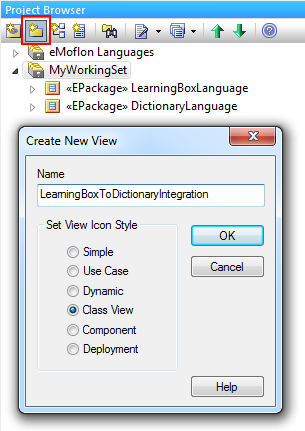
\includegraphics[width=0.5\textwidth]{ea_LearningBoxIntegrationPackage}
  \caption{Create a new TGG integration package}  
  \label{ea:intgPackage}
\end{center}
\end{figure}

\item[$\blacktriangleright$] Create a new  \texttt{TGG Schema} diagram in the new package (Fig.~\ref{ea:tgg_diagram_type}). The diagram type indicates to EA
that the new package is a TGG Project.

\vspace{0.5cm}

\begin{figure}[htbp]
\begin{center}
  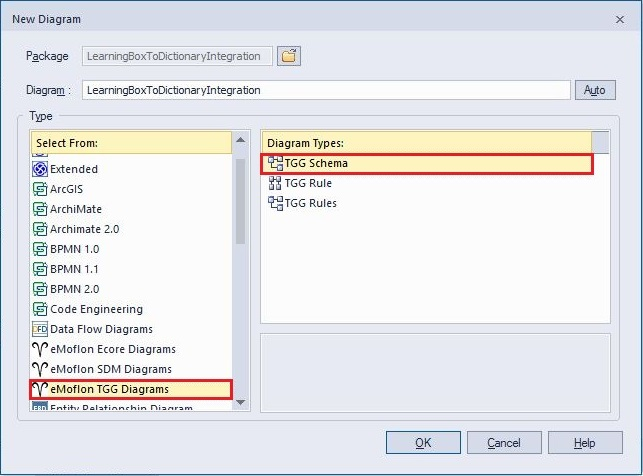
\includegraphics[width=0.9\textwidth]{ea_newTGGSchema}
  \caption{Choose \texttt{TGG Schema} as your diagram type}  
  \label{ea:tgg_diagram_type}
\end{center}
\end{figure}

\item[$\blacktriangleright$] A dialogue should pop up asking to set the source and target projects of the TGG. Set \texttt{Learning\-Box\-Language} as the
source and \texttt{Dictionary\-Language} as the target and affirm with \texttt{OK} (Fig.~\ref{ea:select_source_target}).

\vspace{0.5cm}

\begin{figure}[htbp]
\begin{center}
  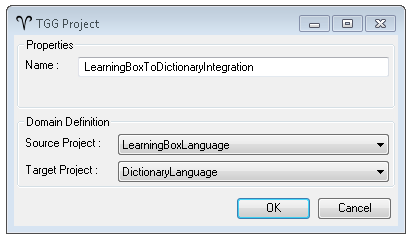
\includegraphics[width=0.55\textwidth]{ea_TGGSourceTarget}
  \caption{Set the \texttt{source} and \texttt{target} projects for the TGG project}  
  \label{ea:select_source_target}
\end{center}
\end{figure}

\item[$\blacktriangleright$] The structure of your TGG project should now resemble Fig.~\ref{ea:new_tgg_project}. Please note that a subpackage \texttt{Rules}
and underlying diagram with the same name are also generated.

\begin{figure}[htbp]
\begin{center}
  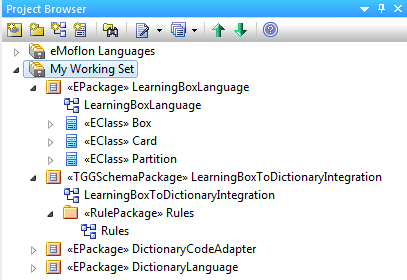
\includegraphics[width=0.5\textwidth]{ea_browserPostDiagram}
  \caption{Initial structure of a new TGG project}  
  \label{ea:new_tgg_project}
\end{center}
\end{figure}
\end{itemize}
\clearpage

\begin{itemize}

\item[$\blacktriangleright$] Now it's time to reference classes from the source and target projects in the TGG project to declare the first \emph{correspondence
type} between them. Confirm the new TGG schema diagram is open in the editor, then hold \texttt{ctrl} and drag-and-drop the \texttt{Box} class from
\texttt{Learning\-Box\-Language} into the window. Paste the class as a simple \texttt{link} into the diagram (Fig.~\ref{ea:TGGdragDrop}). For reference, each
attribute and operation is included in the diagram.\footnote{Take caution: If you press \texttt{ctrl + delete} to delete the element in this diagram,
you will also delete it from its original metamodel package!}

\vspace{0.5cm}

\begin{figure}[htbp]
\begin{center}
  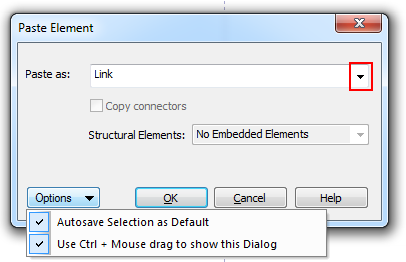
\includegraphics[width=0.6\textwidth]{ea_TGGDragDrop}
  \caption{Copying an element as a simple link} 
  \label{ea:TGGdragDrop}
\end{center}
\end{figure}

\item[$\blacktriangleright$] Note that you are able to set \texttt{Autosave Selection as default}. We'll need to switch drag types several times during this
part, so it's best to leave this unchecked if you do not want to hold \texttt{ctrl} each time you use the drag-and-drop gesture.

\vspace{0.5cm}

\item[$\blacktriangleright$] Repeat the action for a \texttt{Dictionary} from \texttt{DictionaryLanguage} so that you have a class from each metamodel in the
schema.

\vspace{0.5cm}

\item[$\blacktriangleright$] We can now create a correspondence type! Quick-link from \texttt{Box} to \texttt{Dictionary}, selecting \texttt{Create TGG
Corres\-pon\-dence Type} in the context menu (Fig.~\ref{ea:create_correspondence}).

\newpage

\begin{figure}[htbp]
\begin{center}
  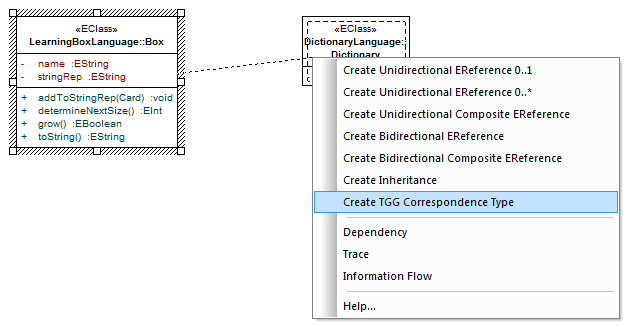
\includegraphics[width=\textwidth]{ea_TGGCorrespType}
  \caption{Quick-link to create a correspondence type} 
  \label{ea:create_correspondence}
\end{center}
\end{figure}

\item[$\blacktriangleright$] As you can see, a correspondence type has been created, visualized as a hexagon (Fig.~\ref{ea:firstCorrType}). It is automatically
named \texttt{BoxToDiction\-ary} and the references are appropriately named.

\vspace{0.5cm}

\begin{figure}[htbp]
\begin{center}
  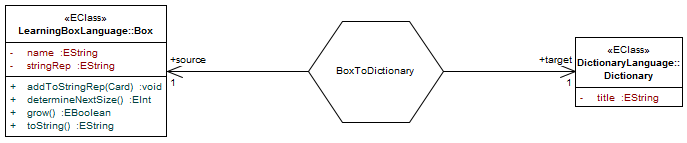
\includegraphics[width=\textwidth]{ea_firstTGGSchema}
  \caption{An established correspondence type} 
  \label{ea:firstCorrType}
\end{center}
\end{figure}

\vspace{0.5cm}

\item[$\blacktriangleright$] You've just finished initalizing your TGG schema! To see how this is done with the textual syntax, check out
Fig.~\ref{eclipse:firstCorrType} in the next section.

% Can this be omitted? Users create a new one on the fly?
% \item[$\blacktriangleright$] To finish our TGG schema, declare a second correspondence type in the same file between \texttt{Card} and \texttt{Entry}. You'll
% notice that the reference between \texttt{Dictionary} and \texttt{Entry} was automatically created! Your completed TGG Schema should resemble
% Fig.~\ref{fig:complete_tgg_schema}.

% \begin{figure}[htbp]
% \begin{center}
%   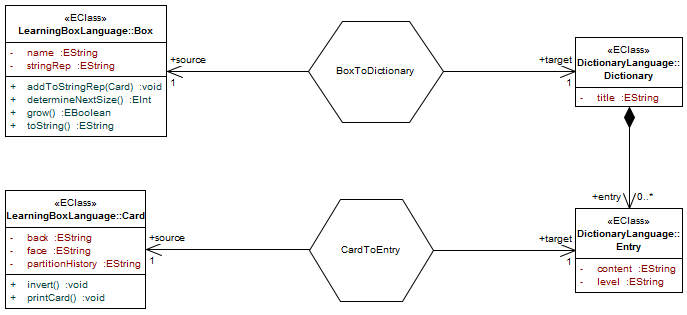
\includegraphics[width=\textwidth]{ea_completeTGGSchema}
%   \caption{Complete TGG schema for our example}
%   \label{fig:complete_tgg_schema}
% \end{center}
% \end{figure}

\jumpSingle{sec:Rules}

\end{itemize}

